% \vspace{-0.25em}
\section{Experiments}
\label{sec:results}
\vspace{-0.25em}

\begin{figure}
  \centering
    \includegraphics[width=\columnwidth]{Figures/COMP3.pdf}
    \vspace{-0.5em}
    \caption{We compare reconstruction quality of our VIN-NBV policy with GenNBV \cite{chen2024gennbv} and ScanRL \cite{peralta2020next} on 3 objects using 20 captures and a modified version of the figure also depicted in the original GenNBV \cite{chen2024gennbv} paper.}
    \label{fig:three_house}
    \vspace{-1em}
\end{figure}

\begin{table}
\vspace{0.75em}
  \centering
    \small
    \begin{tabular}{@{}lc@{}}
      \toprule
      \multicolumn{2}{c}{\textbf{OmniObject3D}} \\
      \midrule
      \textbf{NBV Policy} & Chamfer Distance (cm) $\downarrow$ \\
      \midrule
      Random Hemisphere   & 0.48 \\
      Uniform Hemisphere  & 0.41 \\
      \midrule
      Uncertainty-Guided  & 0.41 \\
      ActiveRMAP, Arxiv'22\cite{zhan2022activermapradiancefieldactive}          & 0.38 \\
      \midrule
      Scan-RL, ECCV'20\cite{peralta2020next} & 0.37 \\
      GenNBV, CVPR'24\cite{chen2024gennbv} & 0.33 \\
      \textbf{VIN-NBV (Ours)}      & \textbf{0.20} \\
      \bottomrule
    \end{tabular}
    \vspace{-0.25em}
    \caption{Quantitative evaluation of NBV policies on OmniObject3D \cite{wu2023omniobject3d} houses (20 acquisitions) using Chamfer Distance. We follow the evaluation setup of GenNBV and report the performance of existing methods from their paper.}
    \label{table:result_chamfer_distance}
  \vspace{0.5em}
\end{table}


We evaluate and compare VIN-NBV to existing NBV approaches that select viewpoints for high-quality 3D reconstructions on standard datasets. We focus on scenarios where an agent can acquire only a few images or has a limited motion time.

\noindent\textbf{Datasets.} We follow the same train-test protocol from GenNBV\cite{chen2024gennbv} by training on a modified subset of Houses3K \cite{peralta2020next}, and testing on the house category from OmniObject3D \cite{wu2023omniobject3d}. We also evaluate on the dinosaur, truck, and animal classes from OmniObject3D \cite{wu2023omniobject3d} to show the generalization beyond the training data (see Section \ref{sec:generalization}). Each object is rendered from 120 views and we begin the acquisition process by selecting the first base view randomly and then set the second base view to be the one closest to the first.

\noindent\textbf{Baselines.} Prior NBV approaches explicitly "look ahead” from hypothetical camera positions by evaluating visibility of the current scene model, either volumetrically by ray-casting through an occupancy/TSDF grid to estimate information gain \cite{Islerinformationgainvolumetric3d, hardouinUAVNBV}, or via rendering-style approximations of coverage from a discrete set of viewpoints \cite{connollydetermination}, with related ray/visibility accounting in sensor-aware formulations \cite{pito1999solution} and quality-driven surface methods \cite{wuqualitydriven}. Following this approach, we design the Coverage-NBV (Cov-NBV) baseline that scores a candidate view by projecting the current 3D reconstruction into its image plane. 

Since our primary goal is to show that our proposed Relative Reconstruction Improvement (RRI) criterion, predicted by the View Introspection Network (VIN), is better than the coverage-based criterion, we use the same sampling-based sequential greedy best next view selection strategy for both VIN-NBV and Cov-NBV. We simply replace the $\mathcal{RRI}$ score (line~\ref{line:score_func} predicted by VIN in Algo.~\ref{method_nbv_algorithm}), with a coverage-based fitness function eq. \ref{eq:cov-fitness1} where $W\times H$ is the image resolution and $\mathbbm{1}(\cdot)$ is an indicator function.

\vspace{-1.0em}
\begin{equation}
Cov(q) =W\times H - \sum_{u=1}^{H} \sum_{v=1}^{W} \mathbbm{1}(C_q(\mathcal{R}_{base})_{u,v})
\label{eq:cov-fitness1}
\end{equation}
\vspace{-0.5em}

This function estimates the number of empty pixels in the query view $C_q$ when rendering the current reconstructed 3D point cloud $\mathcal{R}_{base}$. A higher $Cov(q)$ score suggests that the query view covers more previously unseen areas, making it a potentially valuable viewpoint.
This pixel-space surrogate correlates with reconstruction completeness and serves as a strong, transparent baseline. It is sensor-agnostic, cheap to compute with standard z-buffer rendering, and captures the same “look-ahead visibility” principle that underlies volumetric information-gain methods—without requiring full voxel ray marching.

We also compare our VIN-NBV policy against several existing 3D-based next-best-view (NBV) approaches, including ScanRL \cite{peralta2020next}, GenNBV \cite{chen2024gennbv}, and ActiveRMAP \cite{zhan2022activermapradiancefieldactive}. Since the model weights of GenNBV\cite{chen2024gennbv} are unavailable, we compare with their reported results in the paper directly. We also perform a direct visual comparison to the reconstruction results provided in their paper, as seen in Fig.~\ref{fig:three_house}.

To understand the upper bound performance of our methods in the optimal case we propose Oracle NBV: a variant of the VIN-NBV policy that selects the best image at each step where the fitness function (line~\ref{line:score_func} in Algorithm~\ref{method_nbv_algorithm}) is replaced with the ground-truth Relative Reconstruction Improvement ($\mathcal{RRI}$) of each query view. This method assumes access to the complete ground-truth reconstruction, enabling direct computation of $\mathcal{RRI}$ as defined in Eq.~\ref{eq:rri}. 

For all sampling-based acquisition policies, VIN-NBV, Cov-NBV, and Oracle-NBV, we uniformly render 120 viewpoints in 3 hemispherical shells around the object from which the policies can sample during evaluation.

\noindent\textbf{Metrics.} Since our goal is to improve reconstruction quality, we use the Chamfer Distance as our main accuracy metric, as it can capture fine-grained information at the point level. We also include the coverage percentage and F1 score curves to show the change in reconstruction completeness and quality as more acquisitions are made. For each object, we calculate the metrics between the reconstructed and the ground truth point clouds. We report the average accuracy (Chamfer Distance) in centimeters across all objects in Omniobject3D houses \cite{wu2023omniobject3d}.

\begin{figure}
  \centering
  \includegraphics[width=0.96\columnwidth]{Figures/house_combined_chamfer.pdf}
    \vspace{-1em}
    \caption{
    \textbf{Evaluation with Limited Acquisitions.} Average reconstruction error (in cm) on OmniObject3D \cite{wu2023omniobject3d} houses under constraint on number of acquisitions. VIN-NBV consistently outperforms coverage-based NBV policies.
    }
    \label{fig:chamfer_comparison}
    \vspace{0.5em}
\end{figure}

\subsection{Evaluation with Limited Acquisitions}
\label{limited_capture_results}
\vspace{-0.25em}

To enable direct comparison with GenNBV and ScanRL \cite{qi2023my3dgen, peralta2020next}, we evaluate our policy on the OmniObject3D \cite{wu2023omniobject3d} houses dataset, limited to 20 captures. VIN-NBV outperforms state-of-the-art NBV policies (Table \ref{table:result_chamfer_distance}), achieving an average reconstruction error of 0.20 cm on houses, compared to 0.33 cm for GenNBV \cite{chen2024gennbv} and 0.37 cm for ScanRL. A visual comparison is presented in Fig. \ref{fig:three_house}, modified directly from the final reconstructions presented in the GenNBV \cite{chen2024gennbv} paper, and shows VIN-NBV retains fine detail and overall good reconstruction quality whereas GenNBV and ScanRL produce blurrier results despite good coverage, likely due to the authors' use of mesh renderings as opposed to dense clouds.


In Fig.~\ref{fig:chamfer_comparison} we compare the reconstruction accuracy during the intermediate stages of acquisition between VIN-NBV with the coverage baseline 'Cov-NBV'. We observe that large improvements with respect to the coverage baseline happen during the initial stages of capture, while towards the later stages, both policies result in similar reconstruction quality. Since the model weights and the evaluation code of the GenNBV \cite{chen2024gennbv} paper are unavailable, we were unable to evaluate this method during the intermediate stages of the capture process. The gap between the 'Oracle NBV' and our method shows that there is still room for improvement, especially in the early stages.

\begin{figure}
  \centering
  \begin{subfigure}[b]{0.49\columnwidth}
    \centering
    \includegraphics[width=\linewidth]{Figures/house_mean_coverage_graph.pdf}
    \caption{Coverage \% over captures}
    \label{fig:house_coverage_curve}
  \end{subfigure}\hfill
  \begin{subfigure}[b]{0.49\columnwidth}
    \centering
    \includegraphics[width=\linewidth]{Figures/houses_f1.pdf}
    \caption{F1 score over captures}
    \label{fig:house_fcr_bar}
  \end{subfigure}
  \vspace{-0.5em}
  \caption{%
    \subref{fig:house_coverage_curve} mean coverage percentage and \subref{fig:house_fcr_bar} F1 score across all OmniObject3D house objects at each acquisition step.
  }
  \label{fig:coverage_metrics_two_panel}
  \vspace{0.5em}
\end{figure}


\noindent\textbf{Ablation: Coverage feature $F_{empty}$ in VIN.} To understand the importance of the coverage information we provide with $F_{empty}$, we run an ablation that evaluates the VIN-NBV policy using a VIN trained without $F_{empty}$. In Fig. \ref{fig:chamfer_comparison}, we see that the absence of coverage features makes little difference during the earlier acquisition stages, but is substantial in the later ones. This explains why VIN-NBV achieves large gains over Cov-NBV early on, converging to a similar solution during later stages where coverage is helpful. Although VIN focuses on predicting reconstruction quality, the coverage feature is still a helpful indicator,  which is otherwise hard to learn implicitly during training.

\subsection{Evaluation with Time-Limited Agent Motion}
\label{limited_time_results}
\vspace{-0.25em}

In our time-limited setting, we evaluate our policy under varying constraints on time in motion to understand its efficiency under strict budgets, simulating time-sensitive applications. We assume that the agent is a drone equipped with a depth sensor and camera and travels at a constant velocity of 4 mph, a typical speed for consumer-grade drones. We assume that the drone always takes a straight-line path to the next capture position and determine how far it can travel under different time limits. We use the same OmniObject3D \cite{wu2023omniobject3d} evaluation data as before and scaled all objects to a size of 14 meters to simulate a more realistic capture setting.

\noindent\textbf{Adapting NBV policies for time-limited acquisitions.} At each step during capture, our agent checks how far it can still travel and finds all potential next views that are in range. If our agent is not able to find a next view in range, it stops capturing and computes the Chamfer Distance of the reconstruction with the current captures. We use our VIN-NBV policy to select the NBVs and don't impose a limit on the number of images that the agent can capture.

\begin{figure}
  \centering
  \vspace{-1em}
  \includegraphics[width=0.94\columnwidth]{Figures/time_constraint.pdf}
    \vspace{-1em}
    \caption{
    \textbf{Evaluation with Time-Limited Agent Motion.} Average reconstruction error (in cm) on OmniObject3D \cite{wu2023omniobject3d} houses under constraint on time traversed. VIN-NBV consistently outperforms coverage based NBV policies.
    }
    \label{fig:time_constraint}
    \vspace{0.5em}
\end{figure}

We show results from the time-limited setting in Fig. ~\ref{fig:time_constraint}. Under all time constraints, our method outperforms the coverage baseline, with the largest improvement happening under the strictest time constraints. During the 15-second limit, our method beats the coverage baseline Chamfer Distance by $\sim$25\%. In Fig.~\ref{fig:time_figs}, we visualize the reconstructed 3D scene using our VIN-NBV policy and the coverage baseline (Cov-NBV) for varying time constraints, illustrating that with more time, the policy focuses on capturing views that can fill missing regions and holes in the reconstruction.

\begin{figure}
  \centering
  \vspace{-1.3em}
\includegraphics[width=0.94\columnwidth]{Figures/collision_comparison.pdf}
  \vspace{-1.3em}
    \caption{
        \textbf{Evaluation with Collision Avoidance.} Comparison of average reconstruction error (in cm) on OmniObject3D \cite{wu2023omniobject3d} houses with collisions avoidance planning. VIN-NBV performance is similar while Cov-NBV performance decreases.
    }
    \label{fig:collision_comparison}
    \vspace{0.5em}
\end{figure}

\subsection{Collision Avoidance}
\label{sec:collision_avoidance}
\vspace{-0.25em}

Currently our capture agent assumes that it can perform straight line travel between the current position and the selected next view. This approach does not take into account collisions that may occur from following these straight line trajectories. We demonstrate the ability of our method to handle custom collision criteria by running the evaluation in a setting that requires the selected NBV to have a straight line path that is at least 1 meter away from the reconstruction at all times. In Fig.~\ref{fig:collision_comparison}, we see that even with this additional collision criterion integrated into our NBV-policy, it still performs well and outperforms the Cov-NBV baseline.

\begin{figure*}[!t]
  \centering
  \vspace{-1.0em}
  \begin{subfigure}[t]{0.33\textwidth}
    \centering
    \includegraphics[width=\textwidth]{Figures/dino_combined_chamfer.pdf}
    \caption{Dinosaurs}
    \label{fig:dinosaur_chamf}
  \end{subfigure}
  \hfill
  \begin{subfigure}[t]{0.33\textwidth}
    \centering
    \includegraphics[width=\textwidth]{Figures/motorcycle_combined_chamfer.pdf}
    \caption{Toy Motorcycles}
    \label{fig:motorcycle_chamf}
  \end{subfigure}
  \hfill
  \begin{subfigure}[t]{0.33\textwidth}
    \centering
    \includegraphics[width=\textwidth]{Figures/animal_combined_chamfer.pdf}
    \caption{Toy Animals}
    \label{fig:animal_chamf}
  \end{subfigure}
  \vspace{-0.5em}
  \caption{
  \textbf{Generalization Across Object Categories.} We graph the average Chamfer Distance at each capture stage in three additional object classes namely dinosaurs, toy motorcycles,
  % toy motorcycles, 
  and toy animals. We compare VIN-NBV to a coverage baseline for 20 captures.
  }
  \label{fig:all_generalization}
\end{figure*}

\begin{figure*}[!t]
  \centering
  \vspace{0.25em}
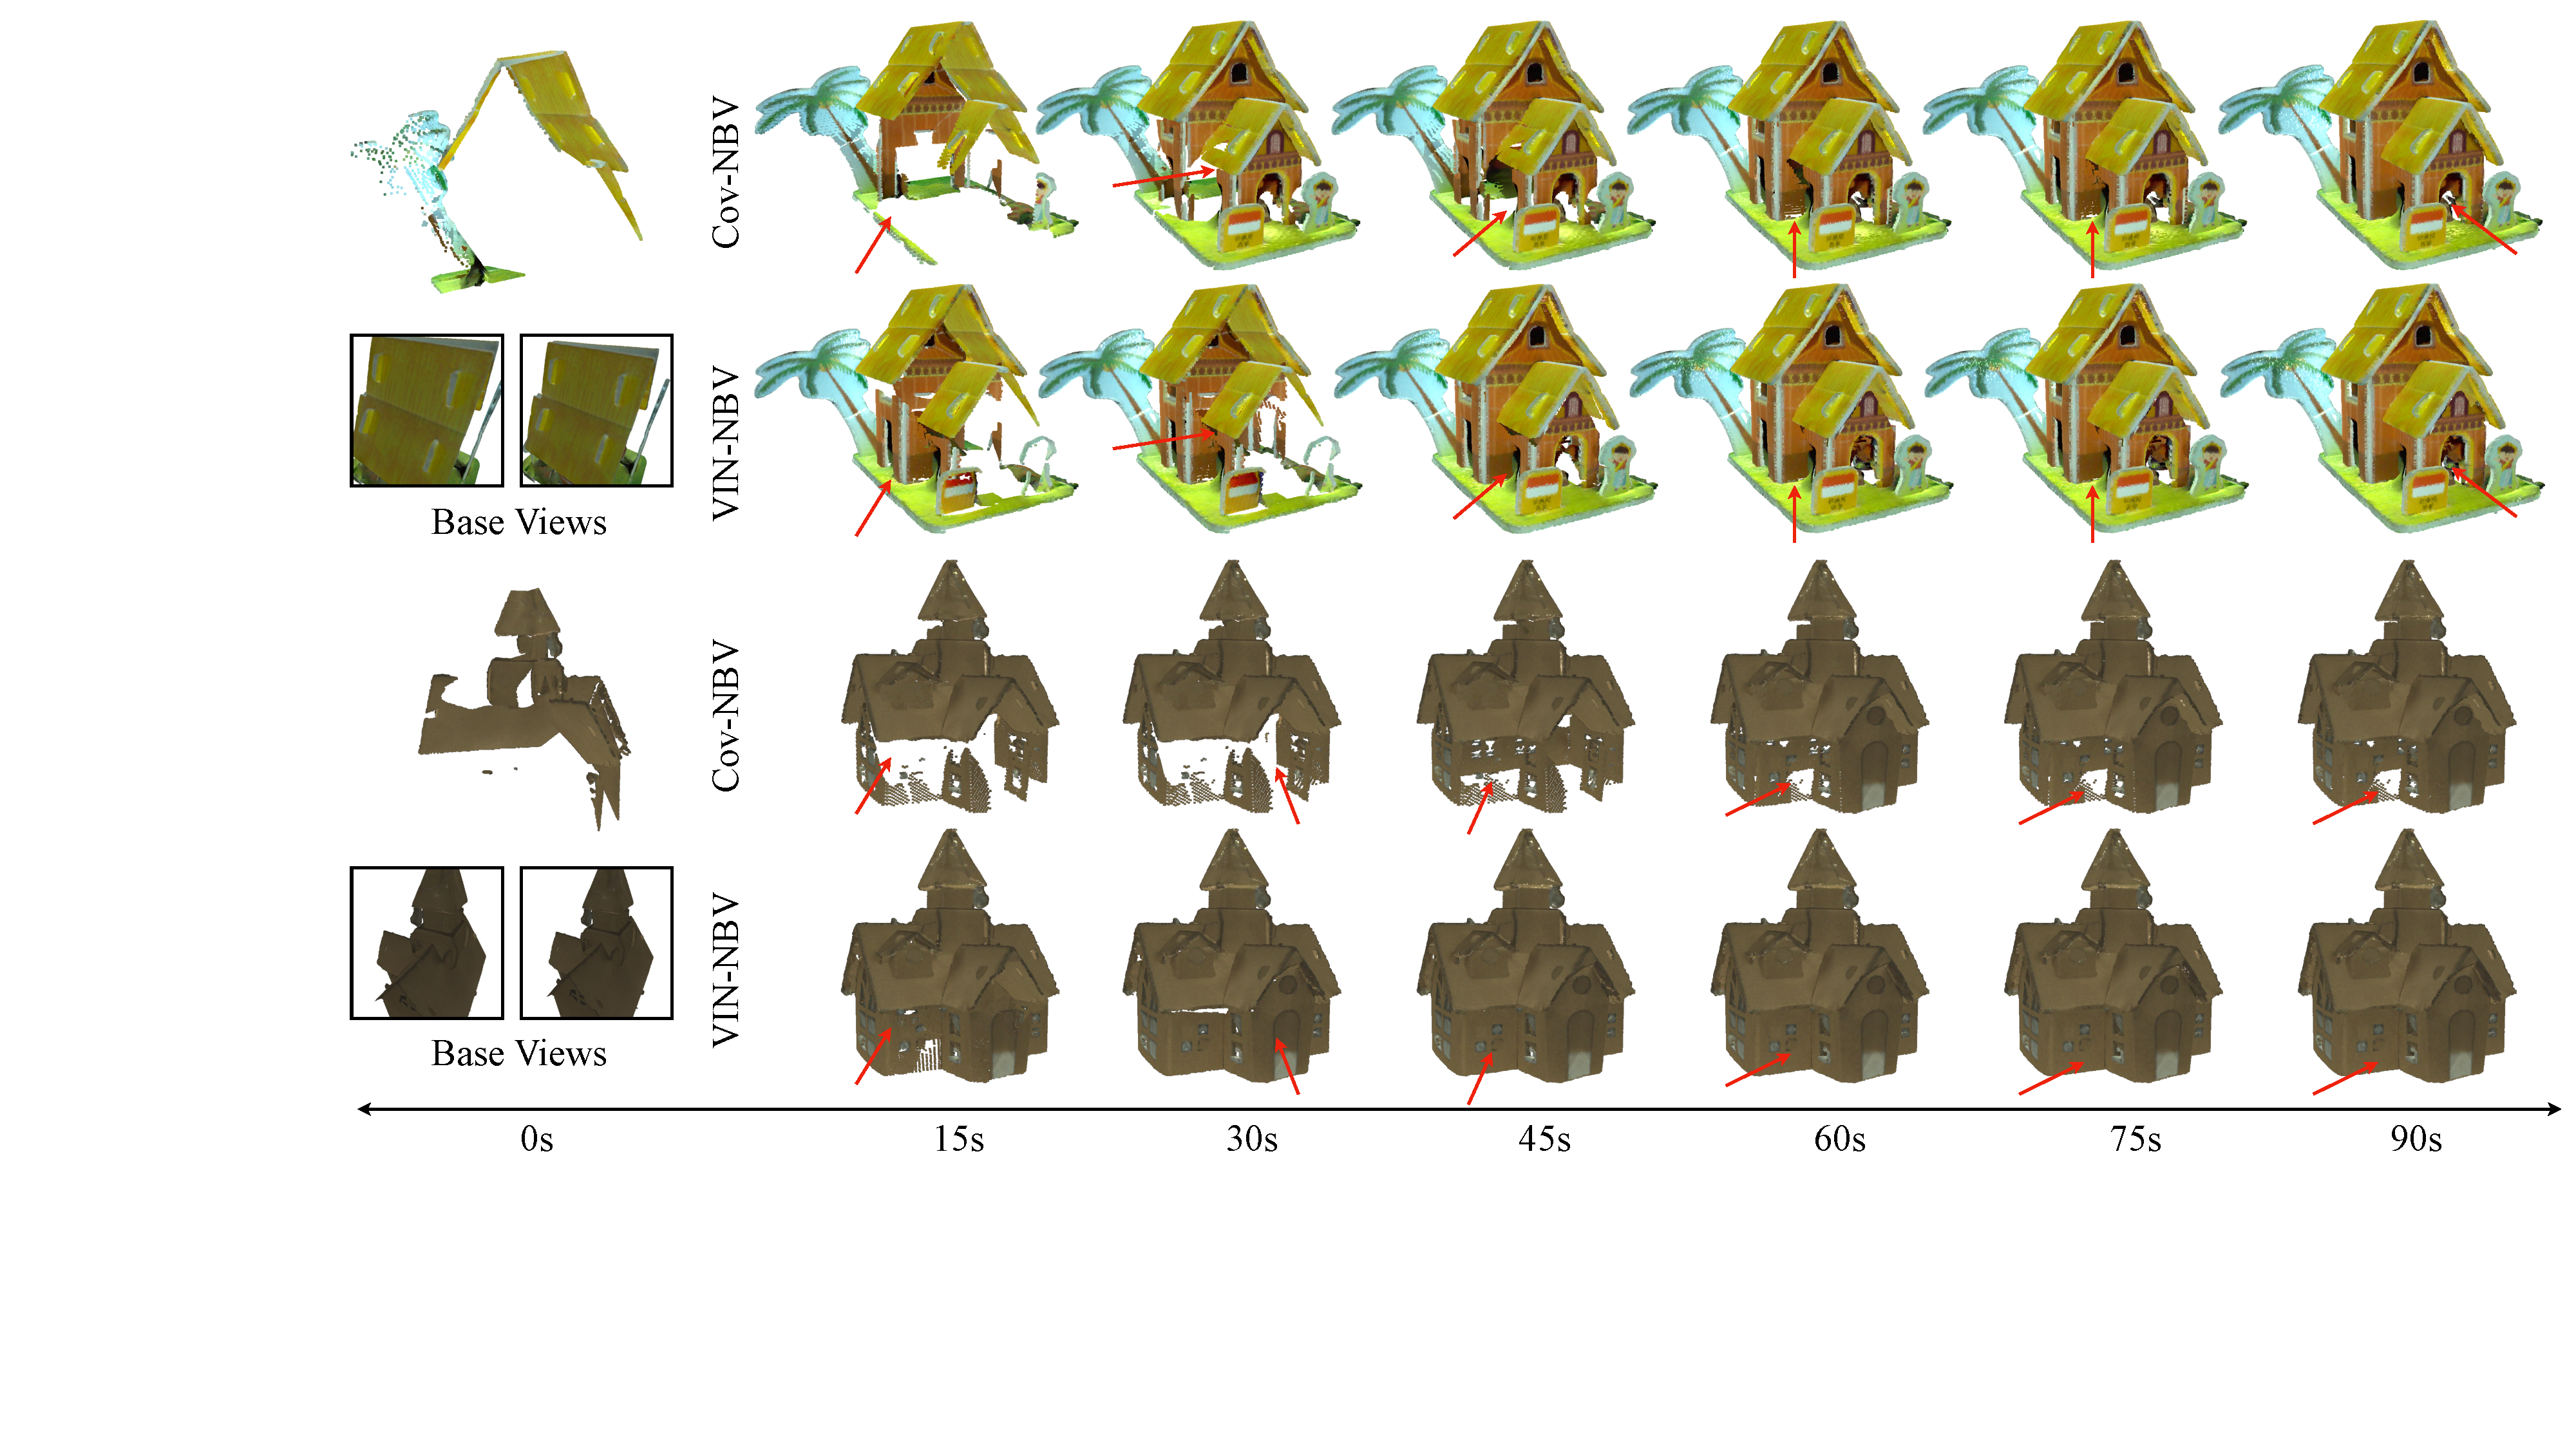
\includegraphics[width=\textwidth]{Figures/time.pdf}
    \vspace{-1.5em}
  \caption{We visualize reconstruction obtained by VIN-NBV and Cov-NBV for different constraints on time traversed. For smaller time budgets, VIN-NBV reconstructions are better with fewer holes.}
  \label{fig:time_figs}
  \vspace{-1.0em}
\end{figure*}

\subsection{Generalization Across Object Categories}
\label{sec:generalization}
\vspace{-0.25em}

We evaluate our policy on additional object categories from OmniObject3D \cite{wu2023omniobject3d}, namely dinosaurs, toy animals, and toy motorcycles. Many of the house objects contain largely planar surfaces with large flat regions and overall less curvature and self-occlusion, in contrast the additional object classes we evaluated have much more detailed surface geometry and instances of self-occlusion. Our results show that even with these new complexities our policy is able to generalize well.

In Fig.\ref{fig:all_generalization} we see that when we evaluate our VIN-NBV policy on additional object categories, it is able to consistently outperform the coverage baseline. Larger gaps in performance occur early on, with both methods reaching similar final Chamfer Distance values at 20 captures. Our policy does particularly well, compared to the coverage baseline, for objects with more complex self-occlusions such as toy motorcycles. We include visual results of our policy and the coverage baseline after 10 acquisitions on several objects and from various viewing angles in Appendix \ref{sec:additional_visuals}.

\begin{table}
\vspace{0.5em}
    \centering
    \begin{tabular}{lccc}
    \toprule
    \textbf{Policy}   & \textbf{Dinosaurs} & \textbf{Trucks} & \textbf{Animals} \\
    \midrule
    Scan-RL \cite{peralta2020next}        & 0.06 & 0.88 & 0.17 \\
    GenNBV \cite{chen2024gennbv}         & \textbf{0.03} & 0.81 & 0.16 \\
    VIN-NBV (ours)       & 0.04   & \textbf{0.57}  & \textbf{0.08}   \\
    \bottomrule
    \end{tabular}
    \vspace{-0.5em}
    \caption{Reconstruction quality comparisons to prior works, with Chamfer Distances ($\downarrow$ is better), on 3 additional classes from OmniObject3D \cite{wu2023omniobject3d} after 20 total acquisitions.}
    \label{table:additional_classes_table}
    \vspace{0.5em}
\end{table}


\vspace{-0.5em}
The toy truck category was also evaluated for final Chamfer Distance so that direct comparisons against GenNBV’s \cite{chen2024gennbv} reported results could be made in Table~\ref{table:additional_classes_table}. VIN-NBV outperforms ScanRL but is slightly behind GenNBV on dinosaurs, while significantly beating both baselines on toy animals and trucks.